
% Default to the notebook output style

    


% Inherit from the specified cell style.




    
\documentclass[11pt]{article}

    
    
    \usepackage[T1]{fontenc}
    % Nicer default font (+ math font) than Computer Modern for most use cases
    \usepackage{mathpazo}

    % Basic figure setup, for now with no caption control since it's done
    % automatically by Pandoc (which extracts ![](path) syntax from Markdown).
    \usepackage{graphicx}
    % We will generate all images so they have a width \maxwidth. This means
    % that they will get their normal width if they fit onto the page, but
    % are scaled down if they would overflow the margins.
    \makeatletter
    \def\maxwidth{\ifdim\Gin@nat@width>\linewidth\linewidth
    \else\Gin@nat@width\fi}
    \makeatother
    \let\Oldincludegraphics\includegraphics
    % Set max figure width to be 80% of text width, for now hardcoded.
    \renewcommand{\includegraphics}[1]{\Oldincludegraphics[width=.8\maxwidth]{#1}}
    % Ensure that by default, figures have no caption (until we provide a
    % proper Figure object with a Caption API and a way to capture that
    % in the conversion process - todo).
    \usepackage{caption}
    \DeclareCaptionLabelFormat{nolabel}{}
    \captionsetup{labelformat=nolabel}

    \usepackage{adjustbox} % Used to constrain images to a maximum size 
    \usepackage{xcolor} % Allow colors to be defined
    \usepackage{enumerate} % Needed for markdown enumerations to work
    \usepackage{geometry} % Used to adjust the document margins
    \usepackage{amsmath} % Equations
    \usepackage{amssymb} % Equations
    \usepackage{textcomp} % defines textquotesingle
    % Hack from http://tex.stackexchange.com/a/47451/13684:
    \AtBeginDocument{%
        \def\PYZsq{\textquotesingle}% Upright quotes in Pygmentized code
    }
    \usepackage{upquote} % Upright quotes for verbatim code
    \usepackage{eurosym} % defines \euro
    \usepackage[mathletters]{ucs} % Extended unicode (utf-8) support
    \usepackage[utf8x]{inputenc} % Allow utf-8 characters in the tex document
    \usepackage{fancyvrb} % verbatim replacement that allows latex
    \usepackage{grffile} % extends the file name processing of package graphics 
                         % to support a larger range 
    % The hyperref package gives us a pdf with properly built
    % internal navigation ('pdf bookmarks' for the table of contents,
    % internal cross-reference links, web links for URLs, etc.)
    \usepackage{hyperref}
    \usepackage{longtable} % longtable support required by pandoc >1.10
    \usepackage{booktabs}  % table support for pandoc > 1.12.2
    \usepackage[inline]{enumitem} % IRkernel/repr support (it uses the enumerate* environment)
    \usepackage[normalem]{ulem} % ulem is needed to support strikethroughs (\sout)
                                % normalem makes italics be italics, not underlines
    

    
    
    % Colors for the hyperref package
    \definecolor{urlcolor}{rgb}{0,.145,.698}
    \definecolor{linkcolor}{rgb}{.71,0.21,0.01}
    \definecolor{citecolor}{rgb}{.12,.54,.11}

    % ANSI colors
    \definecolor{ansi-black}{HTML}{3E424D}
    \definecolor{ansi-black-intense}{HTML}{282C36}
    \definecolor{ansi-red}{HTML}{E75C58}
    \definecolor{ansi-red-intense}{HTML}{B22B31}
    \definecolor{ansi-green}{HTML}{00A250}
    \definecolor{ansi-green-intense}{HTML}{007427}
    \definecolor{ansi-yellow}{HTML}{DDB62B}
    \definecolor{ansi-yellow-intense}{HTML}{B27D12}
    \definecolor{ansi-blue}{HTML}{208FFB}
    \definecolor{ansi-blue-intense}{HTML}{0065CA}
    \definecolor{ansi-magenta}{HTML}{D160C4}
    \definecolor{ansi-magenta-intense}{HTML}{A03196}
    \definecolor{ansi-cyan}{HTML}{60C6C8}
    \definecolor{ansi-cyan-intense}{HTML}{258F8F}
    \definecolor{ansi-white}{HTML}{C5C1B4}
    \definecolor{ansi-white-intense}{HTML}{A1A6B2}

    % commands and environments needed by pandoc snippets
    % extracted from the output of `pandoc -s`
    \providecommand{\tightlist}{%
      \setlength{\itemsep}{0pt}\setlength{\parskip}{0pt}}
    \DefineVerbatimEnvironment{Highlighting}{Verbatim}{commandchars=\\\{\}}
    % Add ',fontsize=\small' for more characters per line
    \newenvironment{Shaded}{}{}
    \newcommand{\KeywordTok}[1]{\textcolor[rgb]{0.00,0.44,0.13}{\textbf{{#1}}}}
    \newcommand{\DataTypeTok}[1]{\textcolor[rgb]{0.56,0.13,0.00}{{#1}}}
    \newcommand{\DecValTok}[1]{\textcolor[rgb]{0.25,0.63,0.44}{{#1}}}
    \newcommand{\BaseNTok}[1]{\textcolor[rgb]{0.25,0.63,0.44}{{#1}}}
    \newcommand{\FloatTok}[1]{\textcolor[rgb]{0.25,0.63,0.44}{{#1}}}
    \newcommand{\CharTok}[1]{\textcolor[rgb]{0.25,0.44,0.63}{{#1}}}
    \newcommand{\StringTok}[1]{\textcolor[rgb]{0.25,0.44,0.63}{{#1}}}
    \newcommand{\CommentTok}[1]{\textcolor[rgb]{0.38,0.63,0.69}{\textit{{#1}}}}
    \newcommand{\OtherTok}[1]{\textcolor[rgb]{0.00,0.44,0.13}{{#1}}}
    \newcommand{\AlertTok}[1]{\textcolor[rgb]{1.00,0.00,0.00}{\textbf{{#1}}}}
    \newcommand{\FunctionTok}[1]{\textcolor[rgb]{0.02,0.16,0.49}{{#1}}}
    \newcommand{\RegionMarkerTok}[1]{{#1}}
    \newcommand{\ErrorTok}[1]{\textcolor[rgb]{1.00,0.00,0.00}{\textbf{{#1}}}}
    \newcommand{\NormalTok}[1]{{#1}}
    
    % Additional commands for more recent versions of Pandoc
    \newcommand{\ConstantTok}[1]{\textcolor[rgb]{0.53,0.00,0.00}{{#1}}}
    \newcommand{\SpecialCharTok}[1]{\textcolor[rgb]{0.25,0.44,0.63}{{#1}}}
    \newcommand{\VerbatimStringTok}[1]{\textcolor[rgb]{0.25,0.44,0.63}{{#1}}}
    \newcommand{\SpecialStringTok}[1]{\textcolor[rgb]{0.73,0.40,0.53}{{#1}}}
    \newcommand{\ImportTok}[1]{{#1}}
    \newcommand{\DocumentationTok}[1]{\textcolor[rgb]{0.73,0.13,0.13}{\textit{{#1}}}}
    \newcommand{\AnnotationTok}[1]{\textcolor[rgb]{0.38,0.63,0.69}{\textbf{\textit{{#1}}}}}
    \newcommand{\CommentVarTok}[1]{\textcolor[rgb]{0.38,0.63,0.69}{\textbf{\textit{{#1}}}}}
    \newcommand{\VariableTok}[1]{\textcolor[rgb]{0.10,0.09,0.49}{{#1}}}
    \newcommand{\ControlFlowTok}[1]{\textcolor[rgb]{0.00,0.44,0.13}{\textbf{{#1}}}}
    \newcommand{\OperatorTok}[1]{\textcolor[rgb]{0.40,0.40,0.40}{{#1}}}
    \newcommand{\BuiltInTok}[1]{{#1}}
    \newcommand{\ExtensionTok}[1]{{#1}}
    \newcommand{\PreprocessorTok}[1]{\textcolor[rgb]{0.74,0.48,0.00}{{#1}}}
    \newcommand{\AttributeTok}[1]{\textcolor[rgb]{0.49,0.56,0.16}{{#1}}}
    \newcommand{\InformationTok}[1]{\textcolor[rgb]{0.38,0.63,0.69}{\textbf{\textit{{#1}}}}}
    \newcommand{\WarningTok}[1]{\textcolor[rgb]{0.38,0.63,0.69}{\textbf{\textit{{#1}}}}}
    
    
    % Define a nice break command that doesn't care if a line doesn't already
    % exist.
    \def\br{\hspace*{\fill} \\* }
    % Math Jax compatability definitions
    \def\gt{>}
    \def\lt{<}
    % Document parameters
    \title{blockchain\_database\_implementation}
    
    
    

    % Pygments definitions
    
\makeatletter
\def\PY@reset{\let\PY@it=\relax \let\PY@bf=\relax%
    \let\PY@ul=\relax \let\PY@tc=\relax%
    \let\PY@bc=\relax \let\PY@ff=\relax}
\def\PY@tok#1{\csname PY@tok@#1\endcsname}
\def\PY@toks#1+{\ifx\relax#1\empty\else%
    \PY@tok{#1}\expandafter\PY@toks\fi}
\def\PY@do#1{\PY@bc{\PY@tc{\PY@ul{%
    \PY@it{\PY@bf{\PY@ff{#1}}}}}}}
\def\PY#1#2{\PY@reset\PY@toks#1+\relax+\PY@do{#2}}

\expandafter\def\csname PY@tok@sx\endcsname{\def\PY@tc##1{\textcolor[rgb]{0.00,0.50,0.00}{##1}}}
\expandafter\def\csname PY@tok@o\endcsname{\def\PY@tc##1{\textcolor[rgb]{0.40,0.40,0.40}{##1}}}
\expandafter\def\csname PY@tok@sd\endcsname{\let\PY@it=\textit\def\PY@tc##1{\textcolor[rgb]{0.73,0.13,0.13}{##1}}}
\expandafter\def\csname PY@tok@cp\endcsname{\def\PY@tc##1{\textcolor[rgb]{0.74,0.48,0.00}{##1}}}
\expandafter\def\csname PY@tok@s1\endcsname{\def\PY@tc##1{\textcolor[rgb]{0.73,0.13,0.13}{##1}}}
\expandafter\def\csname PY@tok@kr\endcsname{\let\PY@bf=\textbf\def\PY@tc##1{\textcolor[rgb]{0.00,0.50,0.00}{##1}}}
\expandafter\def\csname PY@tok@kp\endcsname{\def\PY@tc##1{\textcolor[rgb]{0.00,0.50,0.00}{##1}}}
\expandafter\def\csname PY@tok@il\endcsname{\def\PY@tc##1{\textcolor[rgb]{0.40,0.40,0.40}{##1}}}
\expandafter\def\csname PY@tok@cm\endcsname{\let\PY@it=\textit\def\PY@tc##1{\textcolor[rgb]{0.25,0.50,0.50}{##1}}}
\expandafter\def\csname PY@tok@bp\endcsname{\def\PY@tc##1{\textcolor[rgb]{0.00,0.50,0.00}{##1}}}
\expandafter\def\csname PY@tok@m\endcsname{\def\PY@tc##1{\textcolor[rgb]{0.40,0.40,0.40}{##1}}}
\expandafter\def\csname PY@tok@sa\endcsname{\def\PY@tc##1{\textcolor[rgb]{0.73,0.13,0.13}{##1}}}
\expandafter\def\csname PY@tok@nd\endcsname{\def\PY@tc##1{\textcolor[rgb]{0.67,0.13,1.00}{##1}}}
\expandafter\def\csname PY@tok@c1\endcsname{\let\PY@it=\textit\def\PY@tc##1{\textcolor[rgb]{0.25,0.50,0.50}{##1}}}
\expandafter\def\csname PY@tok@mf\endcsname{\def\PY@tc##1{\textcolor[rgb]{0.40,0.40,0.40}{##1}}}
\expandafter\def\csname PY@tok@ne\endcsname{\let\PY@bf=\textbf\def\PY@tc##1{\textcolor[rgb]{0.82,0.25,0.23}{##1}}}
\expandafter\def\csname PY@tok@gp\endcsname{\let\PY@bf=\textbf\def\PY@tc##1{\textcolor[rgb]{0.00,0.00,0.50}{##1}}}
\expandafter\def\csname PY@tok@gd\endcsname{\def\PY@tc##1{\textcolor[rgb]{0.63,0.00,0.00}{##1}}}
\expandafter\def\csname PY@tok@mh\endcsname{\def\PY@tc##1{\textcolor[rgb]{0.40,0.40,0.40}{##1}}}
\expandafter\def\csname PY@tok@gs\endcsname{\let\PY@bf=\textbf}
\expandafter\def\csname PY@tok@fm\endcsname{\def\PY@tc##1{\textcolor[rgb]{0.00,0.00,1.00}{##1}}}
\expandafter\def\csname PY@tok@sh\endcsname{\def\PY@tc##1{\textcolor[rgb]{0.73,0.13,0.13}{##1}}}
\expandafter\def\csname PY@tok@nt\endcsname{\let\PY@bf=\textbf\def\PY@tc##1{\textcolor[rgb]{0.00,0.50,0.00}{##1}}}
\expandafter\def\csname PY@tok@c\endcsname{\let\PY@it=\textit\def\PY@tc##1{\textcolor[rgb]{0.25,0.50,0.50}{##1}}}
\expandafter\def\csname PY@tok@mb\endcsname{\def\PY@tc##1{\textcolor[rgb]{0.40,0.40,0.40}{##1}}}
\expandafter\def\csname PY@tok@vc\endcsname{\def\PY@tc##1{\textcolor[rgb]{0.10,0.09,0.49}{##1}}}
\expandafter\def\csname PY@tok@nb\endcsname{\def\PY@tc##1{\textcolor[rgb]{0.00,0.50,0.00}{##1}}}
\expandafter\def\csname PY@tok@se\endcsname{\let\PY@bf=\textbf\def\PY@tc##1{\textcolor[rgb]{0.73,0.40,0.13}{##1}}}
\expandafter\def\csname PY@tok@gi\endcsname{\def\PY@tc##1{\textcolor[rgb]{0.00,0.63,0.00}{##1}}}
\expandafter\def\csname PY@tok@nv\endcsname{\def\PY@tc##1{\textcolor[rgb]{0.10,0.09,0.49}{##1}}}
\expandafter\def\csname PY@tok@nf\endcsname{\def\PY@tc##1{\textcolor[rgb]{0.00,0.00,1.00}{##1}}}
\expandafter\def\csname PY@tok@go\endcsname{\def\PY@tc##1{\textcolor[rgb]{0.53,0.53,0.53}{##1}}}
\expandafter\def\csname PY@tok@w\endcsname{\def\PY@tc##1{\textcolor[rgb]{0.73,0.73,0.73}{##1}}}
\expandafter\def\csname PY@tok@si\endcsname{\let\PY@bf=\textbf\def\PY@tc##1{\textcolor[rgb]{0.73,0.40,0.53}{##1}}}
\expandafter\def\csname PY@tok@cs\endcsname{\let\PY@it=\textit\def\PY@tc##1{\textcolor[rgb]{0.25,0.50,0.50}{##1}}}
\expandafter\def\csname PY@tok@vg\endcsname{\def\PY@tc##1{\textcolor[rgb]{0.10,0.09,0.49}{##1}}}
\expandafter\def\csname PY@tok@vm\endcsname{\def\PY@tc##1{\textcolor[rgb]{0.10,0.09,0.49}{##1}}}
\expandafter\def\csname PY@tok@nn\endcsname{\let\PY@bf=\textbf\def\PY@tc##1{\textcolor[rgb]{0.00,0.00,1.00}{##1}}}
\expandafter\def\csname PY@tok@sc\endcsname{\def\PY@tc##1{\textcolor[rgb]{0.73,0.13,0.13}{##1}}}
\expandafter\def\csname PY@tok@kt\endcsname{\def\PY@tc##1{\textcolor[rgb]{0.69,0.00,0.25}{##1}}}
\expandafter\def\csname PY@tok@dl\endcsname{\def\PY@tc##1{\textcolor[rgb]{0.73,0.13,0.13}{##1}}}
\expandafter\def\csname PY@tok@gt\endcsname{\def\PY@tc##1{\textcolor[rgb]{0.00,0.27,0.87}{##1}}}
\expandafter\def\csname PY@tok@vi\endcsname{\def\PY@tc##1{\textcolor[rgb]{0.10,0.09,0.49}{##1}}}
\expandafter\def\csname PY@tok@ss\endcsname{\def\PY@tc##1{\textcolor[rgb]{0.10,0.09,0.49}{##1}}}
\expandafter\def\csname PY@tok@kd\endcsname{\let\PY@bf=\textbf\def\PY@tc##1{\textcolor[rgb]{0.00,0.50,0.00}{##1}}}
\expandafter\def\csname PY@tok@ge\endcsname{\let\PY@it=\textit}
\expandafter\def\csname PY@tok@ni\endcsname{\let\PY@bf=\textbf\def\PY@tc##1{\textcolor[rgb]{0.60,0.60,0.60}{##1}}}
\expandafter\def\csname PY@tok@ow\endcsname{\let\PY@bf=\textbf\def\PY@tc##1{\textcolor[rgb]{0.67,0.13,1.00}{##1}}}
\expandafter\def\csname PY@tok@mo\endcsname{\def\PY@tc##1{\textcolor[rgb]{0.40,0.40,0.40}{##1}}}
\expandafter\def\csname PY@tok@nc\endcsname{\let\PY@bf=\textbf\def\PY@tc##1{\textcolor[rgb]{0.00,0.00,1.00}{##1}}}
\expandafter\def\csname PY@tok@nl\endcsname{\def\PY@tc##1{\textcolor[rgb]{0.63,0.63,0.00}{##1}}}
\expandafter\def\csname PY@tok@k\endcsname{\let\PY@bf=\textbf\def\PY@tc##1{\textcolor[rgb]{0.00,0.50,0.00}{##1}}}
\expandafter\def\csname PY@tok@ch\endcsname{\let\PY@it=\textit\def\PY@tc##1{\textcolor[rgb]{0.25,0.50,0.50}{##1}}}
\expandafter\def\csname PY@tok@sb\endcsname{\def\PY@tc##1{\textcolor[rgb]{0.73,0.13,0.13}{##1}}}
\expandafter\def\csname PY@tok@err\endcsname{\def\PY@bc##1{\setlength{\fboxsep}{0pt}\fcolorbox[rgb]{1.00,0.00,0.00}{1,1,1}{\strut ##1}}}
\expandafter\def\csname PY@tok@gh\endcsname{\let\PY@bf=\textbf\def\PY@tc##1{\textcolor[rgb]{0.00,0.00,0.50}{##1}}}
\expandafter\def\csname PY@tok@gu\endcsname{\let\PY@bf=\textbf\def\PY@tc##1{\textcolor[rgb]{0.50,0.00,0.50}{##1}}}
\expandafter\def\csname PY@tok@kc\endcsname{\let\PY@bf=\textbf\def\PY@tc##1{\textcolor[rgb]{0.00,0.50,0.00}{##1}}}
\expandafter\def\csname PY@tok@s\endcsname{\def\PY@tc##1{\textcolor[rgb]{0.73,0.13,0.13}{##1}}}
\expandafter\def\csname PY@tok@kn\endcsname{\let\PY@bf=\textbf\def\PY@tc##1{\textcolor[rgb]{0.00,0.50,0.00}{##1}}}
\expandafter\def\csname PY@tok@s2\endcsname{\def\PY@tc##1{\textcolor[rgb]{0.73,0.13,0.13}{##1}}}
\expandafter\def\csname PY@tok@sr\endcsname{\def\PY@tc##1{\textcolor[rgb]{0.73,0.40,0.53}{##1}}}
\expandafter\def\csname PY@tok@mi\endcsname{\def\PY@tc##1{\textcolor[rgb]{0.40,0.40,0.40}{##1}}}
\expandafter\def\csname PY@tok@cpf\endcsname{\let\PY@it=\textit\def\PY@tc##1{\textcolor[rgb]{0.25,0.50,0.50}{##1}}}
\expandafter\def\csname PY@tok@gr\endcsname{\def\PY@tc##1{\textcolor[rgb]{1.00,0.00,0.00}{##1}}}
\expandafter\def\csname PY@tok@no\endcsname{\def\PY@tc##1{\textcolor[rgb]{0.53,0.00,0.00}{##1}}}
\expandafter\def\csname PY@tok@na\endcsname{\def\PY@tc##1{\textcolor[rgb]{0.49,0.56,0.16}{##1}}}

\def\PYZbs{\char`\\}
\def\PYZus{\char`\_}
\def\PYZob{\char`\{}
\def\PYZcb{\char`\}}
\def\PYZca{\char`\^}
\def\PYZam{\char`\&}
\def\PYZlt{\char`\<}
\def\PYZgt{\char`\>}
\def\PYZsh{\char`\#}
\def\PYZpc{\char`\%}
\def\PYZdl{\char`\$}
\def\PYZhy{\char`\-}
\def\PYZsq{\char`\'}
\def\PYZdq{\char`\"}
\def\PYZti{\char`\~}
% for compatibility with earlier versions
\def\PYZat{@}
\def\PYZlb{[}
\def\PYZrb{]}
\makeatother


    % Exact colors from NB
    \definecolor{incolor}{rgb}{0.0, 0.0, 0.5}
    \definecolor{outcolor}{rgb}{0.545, 0.0, 0.0}



    
    % Prevent overflowing lines due to hard-to-break entities
    \sloppy 
    % Setup hyperref package
    \hypersetup{
      breaklinks=true,  % so long urls are correctly broken across lines
      colorlinks=true,
      urlcolor=urlcolor,
      linkcolor=linkcolor,
      citecolor=citecolor,
      }
    % Slightly bigger margins than the latex defaults
    
    \geometry{verbose,tmargin=1in,bmargin=1in,lmargin=1in,rmargin=1in}
    
    

    \begin{document}
    
    
    \maketitle
    
    

    
    \begin{Verbatim}[commandchars=\\\{\}]
{\color{incolor}In [{\color{incolor}1}]:} \PY{k+kn}{import} \PY{n+nn}{hashlib}
        \PY{k+kn}{import} \PY{n+nn}{random}
        \PY{k+kn}{import} \PY{n+nn}{json}
\end{Verbatim}


    \section{Transactions, Validation, and updating system
state}\label{transactions-validation-and-updating-system-state}

Blockchain is a distributed database with a set of rules for verifying
new additions. We'll start off by tracking the accounts of two imaginary
people: Alice and Bob, who will trade virtual money with each other.

To simulate a blockchain implementation we need: - initial state showing
the balance of each account - incoming transactions - transaction
validation functionality - transaction blocking functionality - block
validation functionality

\begin{figure}[htbp]
\centering
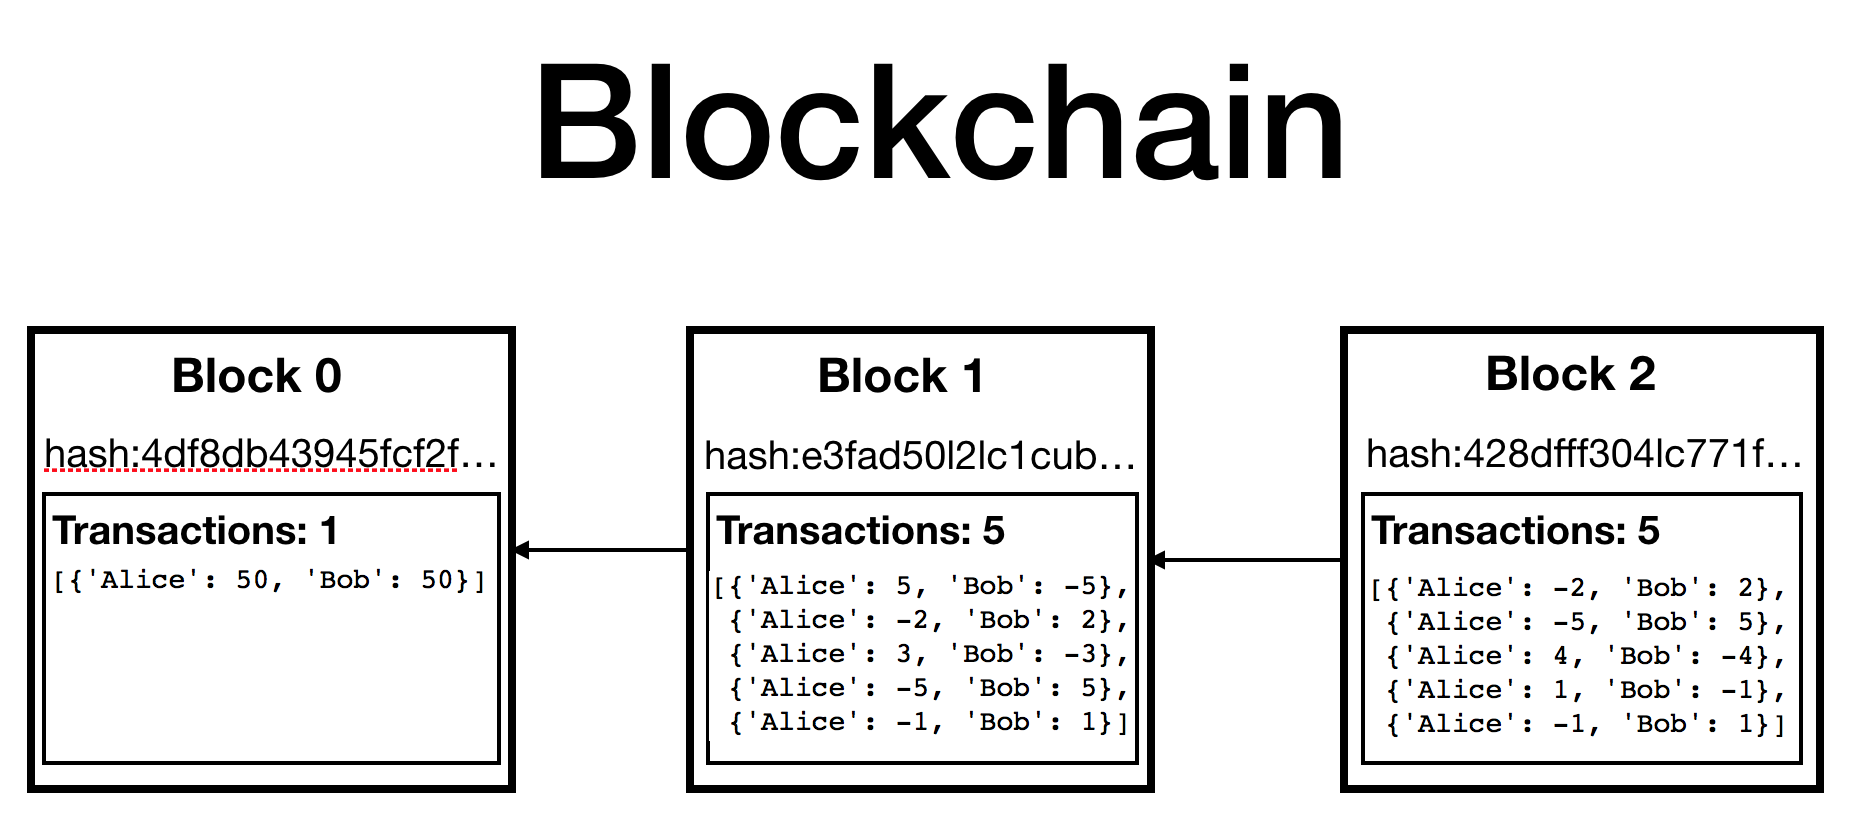
\includegraphics{blockchain.png}
\caption{blockchain}
\end{figure}

    \section{Transactions}\label{transactions}

The function below generates random transactions with rules: -
withdrawal have negative numbers, and deposits positive - deposits have
same magnitude as the withdrawal

    \begin{Verbatim}[commandchars=\\\{\}]
{\color{incolor}In [{\color{incolor}2}]:} \PY{k}{def} \PY{n+nf}{make\PYZus{}random\PYZus{}transaction}\PY{p}{(}\PY{p}{)}\PY{p}{:}
            \PY{n}{amount} \PY{o}{=} \PY{n}{random}\PY{o}{.}\PY{n}{randint}\PY{p}{(}\PY{l+m+mi}{1}\PY{p}{,} \PY{l+m+mi}{5}\PY{p}{)}
            \PY{n}{alice} \PY{o}{=} \PY{n}{random}\PY{o}{.}\PY{n}{choice}\PY{p}{(}\PY{p}{[}\PY{o}{\PYZhy{}}\PY{n}{amount}\PY{p}{,} \PY{n}{amount}\PY{p}{]}\PY{p}{)}
            \PY{n}{bob} \PY{o}{=} \PY{o}{\PYZhy{}}\PY{n}{alice}
            \PY{k}{return} \PY{p}{\PYZob{}}\PY{l+s+s1}{\PYZsq{}}\PY{l+s+s1}{Alice}\PY{l+s+s1}{\PYZsq{}}\PY{p}{:}\PY{n}{alice}\PY{p}{,} \PY{l+s+s1}{\PYZsq{}}\PY{l+s+s1}{Bob}\PY{l+s+s1}{\PYZsq{}}\PY{p}{:}\PY{n}{bob}\PY{p}{\PYZcb{}}
        
        \PY{p}{[}\PY{n}{make\PYZus{}random\PYZus{}transaction}\PY{p}{(}\PY{p}{)} \PY{k}{for} \PY{n}{\PYZus{}} \PY{o+ow}{in} \PY{n+nb}{range}\PY{p}{(}\PY{l+m+mi}{10}\PY{p}{)}\PY{p}{]}
\end{Verbatim}


\begin{Verbatim}[commandchars=\\\{\}]
{\color{outcolor}Out[{\color{outcolor}2}]:} [\{'Alice': -5, 'Bob': 5\},
         \{'Alice': -5, 'Bob': 5\},
         \{'Alice': 3, 'Bob': -3\},
         \{'Alice': 1, 'Bob': -1\},
         \{'Alice': -5, 'Bob': 5\},
         \{'Alice': -5, 'Bob': 5\},
         \{'Alice': -2, 'Bob': 2\},
         \{'Alice': 4, 'Bob': -4\},
         \{'Alice': 3, 'Bob': -3\},
         \{'Alice': -4, 'Bob': 4\}]
\end{Verbatim}
            
    \section{State}\label{state}

    \begin{Verbatim}[commandchars=\\\{\}]
{\color{incolor}In [{\color{incolor}3}]:} \PY{k}{def} \PY{n+nf}{update\PYZus{}state}\PY{p}{(}\PY{n}{transaction}\PY{p}{,} \PY{n}{state}\PY{p}{)}\PY{p}{:}
            \PY{n}{state} \PY{o}{=} \PY{n}{state}\PY{o}{.}\PY{n}{copy}\PY{p}{(}\PY{p}{)}
            \PY{k}{for} \PY{n}{key} \PY{o+ow}{in} \PY{n}{transaction}\PY{p}{:}
                \PY{n}{state}\PY{p}{[}\PY{n}{key}\PY{p}{]} \PY{o}{=} \PY{n}{state}\PY{o}{.}\PY{n}{get}\PY{p}{(}\PY{n}{key}\PY{p}{,} \PY{l+m+mi}{0}\PY{p}{)} \PY{o}{+} \PY{n}{transaction}\PY{p}{[}\PY{n}{key}\PY{p}{]}
            \PY{k}{return} \PY{n}{state}
        
        \PY{n}{state} \PY{o}{=} \PY{p}{\PYZob{}}\PY{l+s+s1}{\PYZsq{}}\PY{l+s+s1}{Alice}\PY{l+s+s1}{\PYZsq{}}\PY{p}{:}\PY{l+m+mi}{5}\PY{p}{,} \PY{l+s+s1}{\PYZsq{}}\PY{l+s+s1}{Bob}\PY{l+s+s1}{\PYZsq{}}\PY{p}{:}\PY{l+m+mi}{5}\PY{p}{\PYZcb{}}
        \PY{n}{transaction} \PY{o}{=} \PY{p}{\PYZob{}}\PY{l+s+s1}{\PYZsq{}}\PY{l+s+s1}{Alice}\PY{l+s+s1}{\PYZsq{}}\PY{p}{:} \PY{o}{\PYZhy{}}\PY{l+m+mi}{3}\PY{p}{,} \PY{l+s+s1}{\PYZsq{}}\PY{l+s+s1}{Bob}\PY{l+s+s1}{\PYZsq{}}\PY{p}{:} \PY{l+m+mi}{3}\PY{p}{\PYZcb{}}
        \PY{n}{state} \PY{o}{=} \PY{n}{update\PYZus{}state}\PY{p}{(}\PY{n}{transaction}\PY{p}{,} \PY{n}{state}\PY{p}{)}
        \PY{n}{state}
\end{Verbatim}


\begin{Verbatim}[commandchars=\\\{\}]
{\color{outcolor}Out[{\color{outcolor}3}]:} \{'Alice': 2, 'Bob': 8\}
\end{Verbatim}
            
    \section{Transaction Validation}\label{transaction-validation}

    \begin{Verbatim}[commandchars=\\\{\}]
{\color{incolor}In [{\color{incolor}4}]:} \PY{k}{def} \PY{n+nf}{validate\PYZus{}transaction}\PY{p}{(}\PY{n}{transaction}\PY{p}{,} \PY{n}{state}\PY{p}{)}\PY{p}{:}
            \PY{k}{if} \PY{n+nb}{sum}\PY{p}{(}\PY{n}{transaction}\PY{o}{.}\PY{n}{values}\PY{p}{(}\PY{p}{)}\PY{p}{)}\PY{p}{:}
                \PY{k}{return} \PY{k+kc}{False}
            
            \PY{k}{for} \PY{n}{key} \PY{o+ow}{in} \PY{n}{transaction}\PY{o}{.}\PY{n}{keys}\PY{p}{(}\PY{p}{)}\PY{p}{:}
                \PY{k}{if} \PY{n}{state}\PY{o}{.}\PY{n}{get}\PY{p}{(}\PY{n}{key}\PY{p}{,} \PY{l+m+mi}{0}\PY{p}{)} \PY{o}{+} \PY{n}{transaction}\PY{p}{[}\PY{n}{key}\PY{p}{]} \PY{o}{\PYZlt{}} \PY{l+m+mi}{0}\PY{p}{:}
                    \PY{k}{return} \PY{k+kc}{False}
        
            \PY{k}{return} \PY{k+kc}{True}
        
        \PY{n}{state} \PY{o}{=} \PY{p}{\PYZob{}}\PY{l+s+s1}{\PYZsq{}}\PY{l+s+s1}{Alice}\PY{l+s+s1}{\PYZsq{}}\PY{p}{:}\PY{l+m+mi}{5}\PY{p}{,} \PY{l+s+s1}{\PYZsq{}}\PY{l+s+s1}{Bob}\PY{l+s+s1}{\PYZsq{}}\PY{p}{:}\PY{l+m+mi}{5}\PY{p}{\PYZcb{}}
        
        \PY{k}{assert} \PY{n}{validate\PYZus{}transaction}\PY{p}{(}\PY{p}{\PYZob{}}\PY{l+s+s1}{\PYZsq{}}\PY{l+s+s1}{Alice}\PY{l+s+s1}{\PYZsq{}}\PY{p}{:} \PY{o}{\PYZhy{}}\PY{l+m+mi}{3}\PY{p}{,} \PY{l+s+s1}{\PYZsq{}}\PY{l+s+s1}{Bob}\PY{l+s+s1}{\PYZsq{}}\PY{p}{:} \PY{l+m+mi}{3}\PY{p}{\PYZcb{}}\PY{p}{,} \PY{n}{state}\PY{p}{)}
        \PY{k}{assert} \PY{o+ow}{not} \PY{n}{validate\PYZus{}transaction}\PY{p}{(}\PY{p}{\PYZob{}}\PY{l+s+s1}{\PYZsq{}}\PY{l+s+s1}{Alice}\PY{l+s+s1}{\PYZsq{}}\PY{p}{:} \PY{o}{\PYZhy{}}\PY{l+m+mi}{4}\PY{p}{,} \PY{l+s+s1}{\PYZsq{}}\PY{l+s+s1}{Bob}\PY{l+s+s1}{\PYZsq{}}\PY{p}{:} \PY{l+m+mi}{3}\PY{p}{\PYZcb{}}\PY{p}{,} \PY{n}{state}\PY{p}{)}
        \PY{k}{assert} \PY{o+ow}{not} \PY{n}{validate\PYZus{}transaction}\PY{p}{(}\PY{p}{\PYZob{}}\PY{l+s+s1}{\PYZsq{}}\PY{l+s+s1}{Alice}\PY{l+s+s1}{\PYZsq{}}\PY{p}{:} \PY{o}{\PYZhy{}}\PY{l+m+mi}{6}\PY{p}{,} \PY{l+s+s1}{\PYZsq{}}\PY{l+s+s1}{Bob}\PY{l+s+s1}{\PYZsq{}}\PY{p}{:} \PY{l+m+mi}{6}\PY{p}{\PYZcb{}}\PY{p}{,} \PY{n}{state}\PY{p}{)}
        \PY{k}{assert} \PY{n}{validate\PYZus{}transaction}\PY{p}{(}\PY{p}{\PYZob{}}\PY{l+s+s1}{\PYZsq{}}\PY{l+s+s1}{Alice}\PY{l+s+s1}{\PYZsq{}}\PY{p}{:} \PY{o}{\PYZhy{}}\PY{l+m+mi}{4}\PY{p}{,} \PY{l+s+s1}{\PYZsq{}}\PY{l+s+s1}{Bob}\PY{l+s+s1}{\PYZsq{}}\PY{p}{:} \PY{l+m+mi}{2}\PY{p}{,} \PY{l+s+s1}{\PYZsq{}}\PY{l+s+s1}{Lisa}\PY{l+s+s1}{\PYZsq{}}\PY{p}{:} \PY{l+m+mi}{2}\PY{p}{\PYZcb{}}\PY{p}{,} \PY{n}{state}\PY{p}{)}
        \PY{k}{assert} \PY{o+ow}{not} \PY{n}{validate\PYZus{}transaction}\PY{p}{(}\PY{p}{\PYZob{}}\PY{l+s+s1}{\PYZsq{}}\PY{l+s+s1}{Alice}\PY{l+s+s1}{\PYZsq{}}\PY{p}{:} \PY{o}{\PYZhy{}}\PY{l+m+mi}{4}\PY{p}{,} \PY{l+s+s1}{\PYZsq{}}\PY{l+s+s1}{Bob}\PY{l+s+s1}{\PYZsq{}}\PY{p}{:} \PY{l+m+mi}{3}\PY{p}{,} \PY{l+s+s1}{\PYZsq{}}\PY{l+s+s1}{Lisa}\PY{l+s+s1}{\PYZsq{}}\PY{p}{:} \PY{l+m+mi}{2}\PY{p}{\PYZcb{}}\PY{p}{,} \PY{n}{state}\PY{p}{)}
\end{Verbatim}


    \section{Blocks}\label{blocks}

Each block contains: - batch of N transactions (N - block size) - a
reference to the hash of the previous block (unless block 0) - block
number - a header with hash of its contents

    \section{Hash function}\label{hash-function}

    \begin{Verbatim}[commandchars=\\\{\}]
{\color{incolor}In [{\color{incolor}5}]:} \PY{k}{def} \PY{n+nf}{hash\PYZus{}function}\PY{p}{(}\PY{n}{msg}\PY{o}{=}\PY{l+s+s1}{\PYZsq{}}\PY{l+s+s1}{\PYZsq{}}\PY{p}{)}\PY{p}{:}
            \PY{k}{if} \PY{n+nb}{type}\PY{p}{(}\PY{n}{msg}\PY{p}{)} \PY{o}{!=} \PY{n+nb}{str}\PY{p}{:}
                \PY{n}{msg} \PY{o}{=} \PY{n}{json}\PY{o}{.}\PY{n}{dumps}\PY{p}{(}\PY{n}{msg}\PY{p}{,} \PY{n}{sort\PYZus{}keys}\PY{o}{=}\PY{k+kc}{True}\PY{p}{)}
            \PY{n}{msg} \PY{o}{=} \PY{n+nb}{str}\PY{p}{(}\PY{n}{msg}\PY{p}{)}\PY{o}{.}\PY{n}{encode}\PY{p}{(}\PY{l+s+s1}{\PYZsq{}}\PY{l+s+s1}{utf\PYZhy{}8}\PY{l+s+s1}{\PYZsq{}}\PY{p}{)}
            \PY{k}{return} \PY{n}{hashlib}\PY{o}{.}\PY{n}{sha256}\PY{p}{(}\PY{n}{msg}\PY{p}{)}\PY{o}{.}\PY{n}{hexdigest}\PY{p}{(}\PY{p}{)}
        
        \PY{n}{hash\PYZus{}function}\PY{p}{(}\PY{p}{\PYZob{}}\PY{l+s+s1}{\PYZsq{}}\PY{l+s+s1}{foo}\PY{l+s+s1}{\PYZsq{}}\PY{p}{:}\PY{l+s+s1}{\PYZsq{}}\PY{l+s+s1}{bar}\PY{l+s+s1}{\PYZsq{}}\PY{p}{\PYZcb{}}\PY{p}{)}
\end{Verbatim}


\begin{Verbatim}[commandchars=\\\{\}]
{\color{outcolor}Out[{\color{outcolor}5}]:} '426fc04f04bf8fdb5831dc37bbb6dcf70f63a37e05a68c6ea5f63e85ae579376'
\end{Verbatim}
            
    \section{Initial State}\label{initial-state}

    \begin{Verbatim}[commandchars=\\\{\}]
{\color{incolor}In [{\color{incolor}6}]:} \PY{n}{state} \PY{o}{=} \PY{p}{\PYZob{}}\PY{l+s+s1}{\PYZsq{}}\PY{l+s+s1}{Alice}\PY{l+s+s1}{\PYZsq{}}\PY{p}{:} \PY{l+m+mi}{50}\PY{p}{,} \PY{l+s+s1}{\PYZsq{}}\PY{l+s+s1}{Bob}\PY{l+s+s1}{\PYZsq{}}\PY{p}{:} \PY{l+m+mi}{50}\PY{p}{\PYZcb{}}
        \PY{n}{blockchain} \PY{o}{=} \PY{p}{[}\PY{p}{]}
\end{Verbatim}


    \section{Block 0 is special}\label{block-0-is-special}

The blockchain is empty and we start by defining the block 0. - not
linked to any prior block - instead of transactions it holds the initial
state

    \begin{Verbatim}[commandchars=\\\{\}]
{\color{incolor}In [{\color{incolor}7}]:} \PY{n}{block0\PYZus{}contents} \PY{o}{=} \PY{p}{\PYZob{}}
            \PY{l+s+s1}{\PYZsq{}}\PY{l+s+s1}{number}\PY{l+s+s1}{\PYZsq{}}\PY{p}{:} \PY{l+m+mi}{0}\PY{p}{,}
            \PY{l+s+s1}{\PYZsq{}}\PY{l+s+s1}{parent\PYZus{}hash}\PY{l+s+s1}{\PYZsq{}}\PY{p}{:} \PY{k+kc}{None}\PY{p}{,}
            \PY{l+s+s1}{\PYZsq{}}\PY{l+s+s1}{transactions\PYZus{}count}\PY{l+s+s1}{\PYZsq{}}\PY{p}{:} \PY{l+m+mi}{1}\PY{p}{,}
            \PY{l+s+s1}{\PYZsq{}}\PY{l+s+s1}{transactions}\PY{l+s+s1}{\PYZsq{}}\PY{p}{:} \PY{p}{[}\PY{n}{state}\PY{p}{]}
        \PY{p}{\PYZcb{}}
        
        \PY{n}{block0} \PY{o}{=} \PY{p}{\PYZob{}}
            \PY{l+s+s1}{\PYZsq{}}\PY{l+s+s1}{hash}\PY{l+s+s1}{\PYZsq{}}\PY{p}{:} \PY{n}{hash\PYZus{}function}\PY{p}{(}\PY{n}{block0\PYZus{}contents}\PY{p}{)}\PY{p}{,}
            \PY{l+s+s1}{\PYZsq{}}\PY{l+s+s1}{contents}\PY{l+s+s1}{\PYZsq{}}\PY{p}{:} \PY{n}{block0\PYZus{}contents}
        \PY{p}{\PYZcb{}}
        
        \PY{n}{blockchain}\PY{o}{.}\PY{n}{append}\PY{p}{(}\PY{n}{block0}\PY{p}{)}
        \PY{n}{blockchain}
\end{Verbatim}


\begin{Verbatim}[commandchars=\\\{\}]
{\color{outcolor}Out[{\color{outcolor}7}]:} [\{'contents': \{'number': 0,
           'parent\_hash': None,
           'transactions': [\{'Alice': 50, 'Bob': 50\}],
           'transactions\_count': 1\},
          'hash': '4df8dbf145fcf2f5ad3f122fa8f33fad4a2498a5325149c3515053fb6b844afd'\}]
\end{Verbatim}
            
    \section{All other blocks are created as
so:}\label{all-other-blocks-are-created-as-so}

    \begin{Verbatim}[commandchars=\\\{\}]
{\color{incolor}In [{\color{incolor}8}]:} \PY{k}{def} \PY{n+nf}{make\PYZus{}block}\PY{p}{(}\PY{n}{transactions}\PY{p}{,} \PY{n}{chain}\PY{p}{)}\PY{p}{:}
            \PY{n}{parent} \PY{o}{=} \PY{n}{chain}\PY{p}{[}\PY{o}{\PYZhy{}}\PY{l+m+mi}{1}\PY{p}{]}
        
            \PY{n}{contents} \PY{o}{=} \PY{p}{\PYZob{}}
                \PY{l+s+s1}{\PYZsq{}}\PY{l+s+s1}{number}\PY{l+s+s1}{\PYZsq{}}\PY{p}{:} \PY{n}{parent}\PY{p}{[}\PY{l+s+s1}{\PYZsq{}}\PY{l+s+s1}{contents}\PY{l+s+s1}{\PYZsq{}}\PY{p}{]}\PY{p}{[}\PY{l+s+s1}{\PYZsq{}}\PY{l+s+s1}{number}\PY{l+s+s1}{\PYZsq{}}\PY{p}{]} \PY{o}{+} \PY{l+m+mi}{1}\PY{p}{,}
                \PY{l+s+s1}{\PYZsq{}}\PY{l+s+s1}{parent\PYZus{}hash}\PY{l+s+s1}{\PYZsq{}}\PY{p}{:} \PY{n}{parent}\PY{p}{[}\PY{l+s+s1}{\PYZsq{}}\PY{l+s+s1}{hash}\PY{l+s+s1}{\PYZsq{}}\PY{p}{]}\PY{p}{,}
                \PY{l+s+s1}{\PYZsq{}}\PY{l+s+s1}{transactions\PYZus{}count}\PY{l+s+s1}{\PYZsq{}}\PY{p}{:} \PY{n+nb}{len}\PY{p}{(}\PY{n}{transactions}\PY{p}{)}\PY{p}{,}
                \PY{l+s+s1}{\PYZsq{}}\PY{l+s+s1}{transactions}\PY{l+s+s1}{\PYZsq{}}\PY{p}{:} \PY{n}{transactions}
            \PY{p}{\PYZcb{}}
            \PY{k}{return} \PY{p}{\PYZob{}}
                \PY{l+s+s1}{\PYZsq{}}\PY{l+s+s1}{hash}\PY{l+s+s1}{\PYZsq{}}\PY{p}{:} \PY{n}{hash\PYZus{}function}\PY{p}{(}\PY{n}{contents}\PY{p}{)}\PY{p}{,}
                \PY{l+s+s1}{\PYZsq{}}\PY{l+s+s1}{contents}\PY{l+s+s1}{\PYZsq{}}\PY{p}{:} \PY{n}{contents}
            \PY{p}{\PYZcb{}}
\end{Verbatim}


    \section{Random transactions for our
blockchain}\label{random-transactions-for-our-blockchain}

    \begin{Verbatim}[commandchars=\\\{\}]
{\color{incolor}In [{\color{incolor}9}]:} \PY{n}{transactions} \PY{o}{=} \PY{p}{[}\PY{n}{make\PYZus{}random\PYZus{}transaction}\PY{p}{(}\PY{p}{)} \PY{k}{for} \PY{n}{\PYZus{}} \PY{o+ow}{in} \PY{n+nb}{range}\PY{p}{(}\PY{l+m+mi}{15}\PY{p}{)}\PY{p}{]}
        \PY{n}{transactions}
\end{Verbatim}


\begin{Verbatim}[commandchars=\\\{\}]
{\color{outcolor}Out[{\color{outcolor}9}]:} [\{'Alice': -5, 'Bob': 5\},
         \{'Alice': 1, 'Bob': -1\},
         \{'Alice': 4, 'Bob': -4\},
         \{'Alice': 5, 'Bob': -5\},
         \{'Alice': -1, 'Bob': 1\},
         \{'Alice': 4, 'Bob': -4\},
         \{'Alice': 5, 'Bob': -5\},
         \{'Alice': -2, 'Bob': 2\},
         \{'Alice': 3, 'Bob': -3\},
         \{'Alice': 5, 'Bob': -5\},
         \{'Alice': -3, 'Bob': 3\},
         \{'Alice': 4, 'Bob': -4\},
         \{'Alice': 2, 'Bob': -2\},
         \{'Alice': 3, 'Bob': -3\},
         \{'Alice': -2, 'Bob': 2\}]
\end{Verbatim}
            
    \section{Create blocks from
transactions}\label{create-blocks-from-transactions}

    \begin{Verbatim}[commandchars=\\\{\}]
{\color{incolor}In [{\color{incolor}10}]:} \PY{n}{block\PYZus{}size} \PY{o}{=} \PY{l+m+mi}{5}
         
         \PY{n}{transactions\PYZus{}buffer} \PY{o}{=} \PY{p}{[}\PY{p}{]}
         \PY{k}{for} \PY{n}{transaction} \PY{o+ow}{in} \PY{n}{transactions}\PY{p}{:}
             \PY{k}{if} \PY{o+ow}{not} \PY{n}{validate\PYZus{}transaction}\PY{p}{(}\PY{n}{transaction}\PY{p}{,} \PY{n}{state}\PY{p}{)}\PY{p}{:}
                 \PY{k}{continue}
                 
             \PY{n}{state} \PY{o}{=} \PY{n}{update\PYZus{}state}\PY{p}{(}\PY{n}{transaction}\PY{p}{,} \PY{n}{state}\PY{p}{)}
             \PY{n}{transactions\PYZus{}buffer}\PY{o}{.}\PY{n}{append}\PY{p}{(}\PY{n}{transaction}\PY{p}{)}
             
             \PY{k}{if} \PY{n+nb}{len}\PY{p}{(}\PY{n}{transactions\PYZus{}buffer}\PY{p}{)} \PY{o}{==} \PY{n}{block\PYZus{}size}\PY{p}{:}
                 \PY{n}{block} \PY{o}{=} \PY{n}{make\PYZus{}block}\PY{p}{(}\PY{n}{transactions\PYZus{}buffer}\PY{p}{,} \PY{n}{blockchain}\PY{p}{)}
                 \PY{n}{blockchain}\PY{o}{.}\PY{n}{append}\PY{p}{(}\PY{n}{block}\PY{p}{)}
                 \PY{n}{transactions\PYZus{}buffer} \PY{o}{=} \PY{p}{[}\PY{p}{]}
         \PY{n}{state}
\end{Verbatim}


\begin{Verbatim}[commandchars=\\\{\}]
{\color{outcolor}Out[{\color{outcolor}10}]:} \{'Alice': 73, 'Bob': 27\}
\end{Verbatim}
            
    \section{Blockchain output}\label{blockchain-output}

    \begin{Verbatim}[commandchars=\\\{\}]
{\color{incolor}In [{\color{incolor}11}]:} \PY{n}{blockchain}
\end{Verbatim}


\begin{Verbatim}[commandchars=\\\{\}]
{\color{outcolor}Out[{\color{outcolor}11}]:} [\{'contents': \{'number': 0,
            'parent\_hash': None,
            'transactions': [\{'Alice': 50, 'Bob': 50\}],
            'transactions\_count': 1\},
           'hash': '4df8dbf145fcf2f5ad3f122fa8f33fad4a2498a5325149c3515053fb6b844afd'\},
          \{'contents': \{'number': 1,
            'parent\_hash': '4df8dbf145fcf2f5ad3f122fa8f33fad4a2498a5325149c3515053fb6b844afd',
            'transactions': [\{'Alice': -5, 'Bob': 5\},
             \{'Alice': 1, 'Bob': -1\},
             \{'Alice': 4, 'Bob': -4\},
             \{'Alice': 5, 'Bob': -5\},
             \{'Alice': -1, 'Bob': 1\}],
            'transactions\_count': 5\},
           'hash': 'db852f505b97b25ba79831ac6d733ffed9051f2af8ef79ed5b8eee5cc2ebb056'\},
          \{'contents': \{'number': 2,
            'parent\_hash': 'db852f505b97b25ba79831ac6d733ffed9051f2af8ef79ed5b8eee5cc2ebb056',
            'transactions': [\{'Alice': 4, 'Bob': -4\},
             \{'Alice': 5, 'Bob': -5\},
             \{'Alice': -2, 'Bob': 2\},
             \{'Alice': 3, 'Bob': -3\},
             \{'Alice': 5, 'Bob': -5\}],
            'transactions\_count': 5\},
           'hash': '6295074487edad26942c90ee1a4cf1a79eb71369f7570daafb9528142a402458'\},
          \{'contents': \{'number': 3,
            'parent\_hash': '6295074487edad26942c90ee1a4cf1a79eb71369f7570daafb9528142a402458',
            'transactions': [\{'Alice': -3, 'Bob': 3\},
             \{'Alice': 4, 'Bob': -4\},
             \{'Alice': 2, 'Bob': -2\},
             \{'Alice': 3, 'Bob': -3\},
             \{'Alice': -2, 'Bob': 2\}],
            'transactions\_count': 5\},
           'hash': '776c583ab2d4e04e2bafaa27deb12654f681fa65a5ad8c341f47a241bf091871'\}]
\end{Verbatim}
            
    \section{Checking Chain Validity}\label{checking-chain-validity}

When we initially set up our blockchain, we have to download the full
blockchain history. After downloading the chain, we would need to run
through the blockchain to compute the state. To protect against somebody
inserting invalid transactions in the initial chain, we need to validate
of the entire chain in this initial download. Once our blockchain is
synced with the network it will need to validate new blocks as they
come.

In order to validate blocks we need the following checks: - block hash
matches the contents - block attributes are valid - all transactions in
block are valid

    \begin{Verbatim}[commandchars=\\\{\}]
{\color{incolor}In [{\color{incolor}12}]:} \PY{k}{def} \PY{n+nf}{validate\PYZus{}block}\PY{p}{(}\PY{n}{block}\PY{p}{,} \PY{n}{parent}\PY{p}{,} \PY{n}{state}\PY{p}{)}\PY{p}{:}    
             \PY{n}{error\PYZus{}msg} \PY{o}{=} \PY{l+s+s1}{\PYZsq{}}\PY{l+s+s1}{Error in }\PY{l+s+si}{\PYZpc{}d}\PY{l+s+s1}{\PYZsq{}} \PY{o}{\PYZpc{}} \PY{n}{block}\PY{p}{[}\PY{l+s+s1}{\PYZsq{}}\PY{l+s+s1}{contents}\PY{l+s+s1}{\PYZsq{}}\PY{p}{]}\PY{p}{[}\PY{l+s+s1}{\PYZsq{}}\PY{l+s+s1}{number}\PY{l+s+s1}{\PYZsq{}}\PY{p}{]}
         
             \PY{c+c1}{\PYZsh{} check block hash}
             \PY{k}{assert} \PY{n}{block}\PY{p}{[}\PY{l+s+s1}{\PYZsq{}}\PY{l+s+s1}{hash}\PY{l+s+s1}{\PYZsq{}}\PY{p}{]} \PY{o}{==} \PY{n}{hash\PYZus{}function}\PY{p}{(}\PY{n}{block}\PY{p}{[}\PY{l+s+s1}{\PYZsq{}}\PY{l+s+s1}{contents}\PY{l+s+s1}{\PYZsq{}}\PY{p}{]}\PY{p}{)}\PY{p}{,} \PY{n}{error\PYZus{}msg}
         
             \PY{c+c1}{\PYZsh{} check block numbers}
             \PY{k}{assert} \PY{n}{block}\PY{p}{[}\PY{l+s+s1}{\PYZsq{}}\PY{l+s+s1}{contents}\PY{l+s+s1}{\PYZsq{}}\PY{p}{]}\PY{p}{[}\PY{l+s+s1}{\PYZsq{}}\PY{l+s+s1}{number}\PY{l+s+s1}{\PYZsq{}}\PY{p}{]} \PY{o}{==} \PY{n}{parent}\PY{p}{[}\PY{l+s+s1}{\PYZsq{}}\PY{l+s+s1}{contents}\PY{l+s+s1}{\PYZsq{}}\PY{p}{]}\PY{p}{[}\PY{l+s+s1}{\PYZsq{}}\PY{l+s+s1}{number}\PY{l+s+s1}{\PYZsq{}}\PY{p}{]} \PY{o}{+} \PY{l+m+mi}{1}\PY{p}{,} \PY{n}{error\PYZus{}msg}
         
             \PY{c+c1}{\PYZsh{} check parent hash}
             \PY{k}{assert} \PY{n}{block}\PY{p}{[}\PY{l+s+s1}{\PYZsq{}}\PY{l+s+s1}{contents}\PY{l+s+s1}{\PYZsq{}}\PY{p}{]}\PY{p}{[}\PY{l+s+s1}{\PYZsq{}}\PY{l+s+s1}{parent\PYZus{}hash}\PY{l+s+s1}{\PYZsq{}}\PY{p}{]} \PY{o}{==} \PY{n}{parent}\PY{p}{[}\PY{l+s+s1}{\PYZsq{}}\PY{l+s+s1}{hash}\PY{l+s+s1}{\PYZsq{}}\PY{p}{]}\PY{p}{,} \PY{n}{error\PYZus{}msg}
             
             \PY{c+c1}{\PYZsh{} check transaction count}
             \PY{k}{assert} \PY{n+nb}{len}\PY{p}{(}\PY{n}{block}\PY{p}{[}\PY{l+s+s1}{\PYZsq{}}\PY{l+s+s1}{contents}\PY{l+s+s1}{\PYZsq{}}\PY{p}{]}\PY{p}{[}\PY{l+s+s1}{\PYZsq{}}\PY{l+s+s1}{transactions}\PY{l+s+s1}{\PYZsq{}}\PY{p}{]}\PY{p}{)} \PY{o}{==} \PY{n}{block}\PY{p}{[}\PY{l+s+s1}{\PYZsq{}}\PY{l+s+s1}{contents}\PY{l+s+s1}{\PYZsq{}}\PY{p}{]}\PY{p}{[}\PY{l+s+s1}{\PYZsq{}}\PY{l+s+s1}{transactions\PYZus{}count}\PY{l+s+s1}{\PYZsq{}}\PY{p}{]}
             
             \PY{c+c1}{\PYZsh{} validate all transactions}
             \PY{k}{for} \PY{n}{transaction} \PY{o+ow}{in} \PY{n}{block}\PY{p}{[}\PY{l+s+s1}{\PYZsq{}}\PY{l+s+s1}{contents}\PY{l+s+s1}{\PYZsq{}}\PY{p}{]}\PY{p}{[}\PY{l+s+s1}{\PYZsq{}}\PY{l+s+s1}{transactions}\PY{l+s+s1}{\PYZsq{}}\PY{p}{]}\PY{p}{:}
                 \PY{k}{assert} \PY{n}{validate\PYZus{}transaction}\PY{p}{(}\PY{n}{transaction}\PY{p}{,} \PY{n}{state}\PY{p}{)}\PY{p}{,} \PY{n}{error\PYZus{}msg}
                 \PY{n}{state} \PY{o}{=} \PY{n}{update\PYZus{}state}\PY{p}{(}\PY{n}{transaction}\PY{p}{,} \PY{n}{state}\PY{p}{)}
                 
             \PY{k}{return} \PY{n}{state}
\end{Verbatim}


    \section{Blockchain initialization}\label{blockchain-initialization}

    \begin{Verbatim}[commandchars=\\\{\}]
{\color{incolor}In [{\color{incolor}13}]:} \PY{k}{def} \PY{n+nf}{check\PYZus{}chain}\PY{p}{(}\PY{n}{blockchain}\PY{p}{)}\PY{p}{:}
             \PY{n}{state} \PY{o}{=} \PY{p}{\PYZob{}}\PY{p}{\PYZcb{}}
         
             \PY{k}{for} \PY{n}{transaction} \PY{o+ow}{in} \PY{n}{blockchain}\PY{p}{[}\PY{l+m+mi}{0}\PY{p}{]}\PY{p}{[}\PY{l+s+s1}{\PYZsq{}}\PY{l+s+s1}{contents}\PY{l+s+s1}{\PYZsq{}}\PY{p}{]}\PY{p}{[}\PY{l+s+s1}{\PYZsq{}}\PY{l+s+s1}{transactions}\PY{l+s+s1}{\PYZsq{}}\PY{p}{]}\PY{p}{:}
                 \PY{n}{state} \PY{o}{=} \PY{n}{update\PYZus{}state}\PY{p}{(}\PY{n}{transaction}\PY{p}{,} \PY{n}{state}\PY{p}{)}
         
             \PY{n}{parent} \PY{o}{=} \PY{n}{blockchain}\PY{p}{[}\PY{l+m+mi}{0}\PY{p}{]}
             
             \PY{k}{for} \PY{n}{block} \PY{o+ow}{in} \PY{n}{blockchain}\PY{p}{[}\PY{l+m+mi}{1}\PY{p}{:}\PY{p}{]}\PY{p}{:}
                 \PY{n}{state} \PY{o}{=} \PY{n}{validate\PYZus{}block}\PY{p}{(}\PY{n}{block}\PY{p}{,} \PY{n}{parent}\PY{p}{,} \PY{n}{state}\PY{p}{)}
                 \PY{n}{parent} \PY{o}{=} \PY{n}{block}
         
             \PY{k}{return} \PY{n}{state}
         
         \PY{n}{check\PYZus{}chain}\PY{p}{(}\PY{n}{blockchain}\PY{p}{)}
\end{Verbatim}


\begin{Verbatim}[commandchars=\\\{\}]
{\color{outcolor}Out[{\color{outcolor}13}]:} \{'Alice': 73, 'Bob': 27\}
\end{Verbatim}
            
    \section{Conclusions}\label{conclusions}

We've created all the basic architecture for a blockchain, from a set of
state transition rules to a method for creating blocks, to mechanisms
for checking the validity of transactions, blocks, and the full chain.
We can derive the system state from a downloaded copy of the blockchain,
validate new blocks that we receive from the network, and create our own
blocks.

    \section{Extensions}\label{extensions}

We haven't explored the network architecture, the proof-of-work or
proof-of-state validation step, and the consensus mechanism which
provides blockchains with security against attack. We also haven't
discussed public key cryptography, privacy, and verification steps.

    \section{References}\label{references}

\begin{itemize}
\tightlist
\item
  https://github.com/post2web/basic\_blockchain
\item
  http://ecomunsing.com/build-your-own-blockchain
\item
  http://www.androidauthority.com/what-is-a-blockchain-gary-explains-801514/
\end{itemize}


    % Add a bibliography block to the postdoc
    
    
    
    \end{document}
